\capitulo{5}{Aspectos relevantes del desarrollo del proyecto}

Este apartado recoge los aspectos más interesantes del desarrollo del trabajo.


\section{Metodologías}

\subsection{Metodologías ágiles(\href{https://www.scrum.org/}{SCRUM})}
Scrum es un marco de trabajo ágil utilizado comúnmente en el desarrollo de software, 
aunque se ha extendido a otras áreas. \\
Proporciona un enfoque estructurado para la gestión de proyectos que se centra en la entrega 
iterativa y incremental de productos. \\
Scrum se basa en los principios del manifiesto ágil y busca mejorar la eficiencia, 
la flexibilidad y la colaboración en equipos de desarrollo.

\subsubsection{Roles}

\begin{itemize}
   \item \textbf{Scrum Master}: facilita el proceso Scrum, elimina obstáculos y ayuda al equipo a alcanzar sus objetivos.
   \item \textbf{Product Owner}: representa las necesidades del cliente y define las características del producto.
   \item \textbf{Equipo de Desarrollo}: profesionales que trabajan en la entrega del producto.
\end{itemize}

\subsubsection{Eventos}

\begin{itemize}
   \item \textbf{Sprint}: un periodo de tiempo fijo (generalmente de 2 a 4 semanas) en el que se entrega un incremento de producto.
   \item \textbf{Reunión de Planificación del Sprint}: al inicio de cada sprint, el equipo planifica el trabajo que se realizará durante ese periodo.
   \item \textbf{Revisión del Sprint}: al final de cada sprint, el equipo presenta el trabajo completado al Product Owner y a otras partes interesadas.
   \item \textbf{Retrospectiva del Sprint}: una sesión al final de cada sprint donde el equipo revisa su desempeño y busca formas de mejorar.
\end{itemize}

\subsubsection{Artefactos}

\begin{itemize}
\item \textbf{Product Backlog}: una lista priorizada de todas las funcionalidades, cambios y mejoras propuestas para el producto.
\item \textbf{Sprint Backlog}: la lista de tareas que el equipo se compromete a completar durante un sprint.
\item \textbf{Incremento}: el producto funcional y potencialmente entregable al final de cada sprint.
\end{itemize}

Scrum promueve la transparencia, la inspección y la adaptación, lo que significa que los equipos pueden ajustar su enfoque y estrategia en función de los cambios en los requisitos del cliente o en las circunstancias del proyecto. Este marco de trabajo es especialmente útil en entornos donde los requisitos pueden cambiar con frecuencia y se valora la capacidad de respuesta y flexibilidad del equipo de desarrollo.

Para este proyecto se ha seguido la metodología \textbf{SCRUM} configurando los sprints con una duración de 2 semanas,
para la planificación se ha utilizado la herramienta \href{https://zube.io/tgs1003/tfg_2023_2024}{Zube}.
Se puede encontrar más detalles sobre el proceso seguido en los anexos de este documento.

\subsection{DevOps~\cite{devops}}
\textbf{DevOps} es una cultura, filosofía y conjunto de prácticas que se centran en la colaboración 
estrecha y la integración continua entre los equipos de desarrollo (Dev) y operaciones (Ops) 
en el ciclo de vida del desarrollo de software. \\
El objetivo principal de \textbf{DevOps} es acelerar la entrega de software, 
mejorar la calidad y la confiabilidad, y permitir una respuesta rápida a los 
cambios y a las necesidades de los usuarios. \\DevOps promueve la automatización, 
la comunicación eficaz y la colaboración entre los equipos, lo que permite un flujo 
de trabajo más eficiente en todo el proceso de desarrollo y entrega de software.\\
Algunos de los principios y prácticas clave de \textbf{DevOps} son:
\begin{itemize}
   \item \textbf{Automatización}: la automatización de tareas repetitivas y procesos manuales acelera la entrega y minimiza los errores. Esto incluye la automatización de pruebas, implementaciones, aprovisionamiento de infraestructura y monitoreo.
   \item \textbf{Integración Continua (CI)}: los cambios de código se integran regularmente en un repositorio compartido, 
se prueban automáticamente y se implementan en un entorno de desarrollo o de prueba. 
Esto asegura que el código esté siempre en un estado funcional.
\item \textbf{Entrega Continua (CD)}: la entrega continua extiende la integración continua al permitir 
la entrega automática de cambios a entornos de prueba o producción después de la integración y 
las pruebas exitosas.
\item \textbf{Monitoreo y Retroalimentación Continua}: el monitoreo constante de aplicaciones y sistemas 
permite detectar problemas en tiempo real y proporciona información valiosa para 
mejorar la calidad y la eficiencia.
\item \textbf{Colaboración y Comunicación}: la comunicación efectiva entre los equipos de desarrollo y 
operaciones es esencial. La colaboración se fomenta mediante reuniones regulares, 
herramientas compartidas y un entendimiento mutuo de las metas y responsabilidades.
\item \textbf{Infraestructura como Código (IaC)}: la infraestructura se administra y despliega como código, 
lo que facilita la creación y el mantenimiento de entornos de desarrollo y producción 
consistentes y escalables.
\item \textbf{Cultura de Mejora Continua}: DevOps promueve una cultura en la que se aprende 
de los errores y se busca constantemente la mejora en todos los aspectos del desarrollo y 
la operación de software.
\item \textbf{Seguridad}: la seguridad es un aspecto crítico de \textbf{DevOps}. 
Los principios de seguridad deben estar integrados en todas las etapas 
del ciclo de vida del desarrollo de software.
\end{itemize}
La implementación de \textbf{DevOps} puede llevar a una mayor velocidad de entrega, 
una mayor calidad del software, una mayor eficiencia operativa y 
una mayor capacidad de respuesta a los cambios del mercado y las necesidades del cliente. 
Esta metodología se ha vuelto esencial en el desarrollo de software moderno, 
especialmente en entornos ágiles y de entrega continua.

Para el publicar del código de este trabajo se ha utilizado \href{https://www.docker.com/}{Docker} 
junto con \href{https://www.portainer.io/}{Portainer}  y \href{https:\\www.github.com}{Github} para el 
despliegue continuo.


\section{Desarrollo del proyecto}

El principal escollo que me he encontrado para la realización de este proyecto es la elección del modelo
LLM adecuado. \\
Por un lado tenemos el servicio de \href{https://openai.com}{OpenAI}. Este servicio es quizá el más estable y que 
mejores resultados obtiene.\\ 
Sin embargo este servicio es de pago (aunque propocionan un saldo gratuito al crear una cuenta, 
no permite realizar más de 3 llamadas al minuto).
Además tenemos el tiempo de proceso para cada reseña (unos 3 segundos).
Existe otros LLMs disponibles como por ejemplo \href{https://ai.meta.com/}{Llama2 (Meta)}, 
\href{https://bard.google.com/chat}{Bard(Google)}.\\
Con el modelo de Meta existe la posibilidad de ejecutarlo en un entorno local mediante 
diferentes librerías (LlamaCpp).\\
Otros modelos que se pueden ejecutar en local son \href{https://gpt4all.io/index.html}{GPT4All}.
Una herramienta muy útil para elegir el modelo adecuado es \href{https://lmstudio.ai/}{LM Studio}, permite descargar y probar distintos modelos,
además ofrece una API compatible con OpenAI.\\
Para la ejecución en local es muy recomendable el uso de una tarjeta gráfica 
para optimizar la ejecución del modelo.

Al planificar el segundo sprint incluí una tarea para crear un prototipo en collab, 
sin embargo esta tarea tenía unas dependencias que hacían imposible su realización.
Lo primero que tenía que hacer era seleccionar un dataset para poder realizar las pruebas.
Y además necesitaba seleccionar el modelo LLM idóneo para la realización de este protoripo.
Una vez replanificadas las tareas en el orden adecuado, seleccioné un conjunto de datos de huggingface y 
un modelo LLM basado en LlamaCpp para usarlo en el notebook de collab.
Al usar un modelo basado en LlamaCpp la ejecución resulta más lenta (unos 30 segundos por reseña) 
pero no se infiere en costes de proceso.


\section{Elección del conjunto de datos}

Elegir un conjunto de datos adecuado es crucial para el análisis de sentimientos.
En este proyecto nos insteresa realizar un análisis de sentimientos en reseñas de 
Amazon por lo que se ha buscado con esa premisa. \\
Esto reduce la búsqueda pero aun así hay que encontrar 
un conjunto de datos que tenga una serie de características que lo haga ideal para su uso en el proyecto.\\
Por un lado, como veremos más adelante, el análisis de sentimiento tiene un coste, 
ya sea económico (OpenAI), o en tiempo (LlamaCpp).
Esto implica que tenemos que elegir un dataset de un tamaño adecuado.
Por un lado, tiene que ser suficientemente grande para que los resultados sean significativos y 
por otro lado lo suficientemente pequeño como para que el coste sea adecuado al proyecto.
El conjunto de datos debe contener información suficiente como para poder realizar 
comparaciones bajo distintas circustancias de estudio, por usuario, por producto, etc.\\
También sería interesante que el conjunto de datos sea represativo de la población, 
para ello lo ideal sería obtener el conjunto de datos de diferentes orígenes.\\
En nuestro caso el origen es siempre Amazon pero a la hora de seleccionar los datos 
intentaremos que estos sean lo más variados posibles.\\
Además hay tener en cuenta la disponibilidad, en algunos casos Amazon ha decidido anular 
la licencia de uso con lo que esos conjuntos de datos no se podrían usar.\\
En base a estas premisas se han estudiado datasets de diferentes orígenes:

\subsection{Universidad de California~\cite{jin018}}
La Universidad de California proporciona un conjunto de datos con reseñas de Amazon. Los más llamativo de este conjunto de datos es su tamaño (230 millones de reseñas) y la cantidad de metadatos incluidos.
También propocionan ejemplos de uso y de código así como un cuaderno en \href{https://colab.research.google.com/drive/1Zv6MARGQcrBbLHyjPVVMZVnRWsRnVMpV}{Colab}.
\par
\href{https://cseweb.ucsd.edu/~jmcauley/datasets/amazon_v2/}{Amazon Reviews Dataset}

\subsection{Kaggle}
Kaggle es una plataforma en línea que ofrece una variedad de recursos relacionados con la ciencia de datos y el aprendizaje automático. Fue fundada en 2010 y adquirida por Google en 2017. Kaggle proporciona un entorno donde los científicos de datos, los investigadores y los entusiastas del aprendizaje automático pueden colaborar, compartir conocimientos, participar en competiciones de ciencia de datos y acceder a conjuntos de datos.
Uno de los conjuntos de datos evaluados han sido:
\begin{itemize}
   \item \href{https://www.kaggle.com/datasets/bittlingmayer/amazonreviews}{Amazon Reviews for Sentiment Analysis}
   \par Este conjuntos de datos tiene un tamaño adecuado para nuestro proposito pero le faltan metadatos y no nos permitiría desarrollar toda la funcionalidad esperada en la aplicación.
   \item \href{https://www.kaggle.com/datasets/kritanjalijain/amazon-reviews}{Amazon Reviews}
\end{itemize}

\subsection{Hugging Face}
Hugging Face es una empresa y plataforma en línea que se centra en la creación y distribución de modelos de lenguaje de inteligencia artificial, así como en herramientas y recursos relacionados con el procesamiento del lenguaje natural (NLP). La compañía es conocida por su biblioteca de modelos preentrenados, así como por su contribución a la comunidad de aprendizaje automático y NLP.
Existen muchos conjuntos de datos que podemos usar para nuestro proyecto, por ejemplo:
\begin{itemize}
   \item \href{https://huggingface.co/datasets/mesmalif/amazon-shoe-reviews}{Amazon Shoe Reviews}
   \item \href{https://huggingface.co/datasets/LoganKells/amazon_product_reviews_video_games}{Amazon Video Games Review}
   \item \href{https://huggingface.co/datasets/hugginglearners/amazon-reviews-sentiment-analysis}{Amazon Reviews for Sentiment Analysis}   
\end{itemize}

Finalmente se ha utilizado un conjunto de datos de huggingface, ya que contiente más metadatos que han resultado útiles
para la organización de las pruebas (Amazon Shoe Reviews).
Por otro lado se han preparado una serie de ficheros con reseñas para poder hacer la demostración.
Tanto el fichero python para preparar esos fichero como los ficheros en sí, se pueden encontrar en la 
carpeta datasets del repositorio de código.

\section{Elección del modelo LLM}

Para la elección del modelo a usar en este trabajo, primero examinamos el modelo más sencillo de utilizar.
Este es el modelo de OpenAI~\cite{chatgpt1}. En concreto el modelo \textbf{ChatGpt 3.5 Turbo}, este modelo es muy estable, rápido y económico.
El problema de usar este modelo, a pesar de ser económico, es su coste.
Para evitar ese problema y poder utilizar un modelo sin limitaciones, he buscado otras alternativas.
Entre estas se encuentran:
\begin{itemize}
   \item \textbf{Microsoft Azure Language Models}: Microsoft Azure ofrece varios servicios de procesamiento del lenguaje natural, incluidos modelos de lenguaje como parte de su oferta de servicios cognitivos.
   \item \textbf{Google Cloud Natural Language API}: Google Cloud proporciona una API de procesamiento del lenguaje natural que incluye funciones avanzadas como análisis de sentimientos, extracción de entidades y más.
   \item \textbf{Hugging Face Transformers}: Hugging Face es una plataforma que ofrece acceso a una amplia variedad de modelos de lenguaje preentrenados. Los modelos GPT y otros están disponibles a través de su biblioteca Transformers.
   \item \textbf{Facebook AI}: Facebook AI Research (FAIR) trabaja en el desarrollo de modelos de lenguaje y herramientas relacionadas con la inteligencia artificial. Aunque no tienen un modelo específico comparable a GPT, han contribuido significativamente al campo.
   \item \textbf{Rasa}: Rasa es una plataforma de código abierto para construir asistentes conversacionales. Permite a los desarrolladores crear chatbots personalizados y asistentes virtuales.
   \item \textbf{Chatbot Frameworks} hºay varios marcos y bibliotecas de código abierto que permiten a los desarrolladores construir sus propios chatbots, como ChatterBot, Botpress, y Microsoft Bot Framework.
   \item \textbf{Dialogflow}: Dialogflow, propiedad de Google, es una plataforma de desarrollo de chatbots y asistentes virtuales que utiliza tecnologías de procesamiento del lenguaje natural.
\end{itemize}

Investigando sobre las diferentes alternativas nos hemos encontrado con 
dificultades a la hora de elegir la idónea.
Por un lado, están los modelos que también son de pago como son ``Microsoft Azure Language Models'' 
y Google Cloud Natural Language API. Ambas soluciones ofrecen periodos de prueba limitados.
Por otro lado están las plataformas para asistentes conversacionales como Dialogflow, Rasa, etc 
que no ofrecen un API para poder usarlas en un programa.
Por último nos queda \textbf{Facebook API}, en este caso su modelo 
\href{https://github.com/facebookresearch/llama}{Llama2} está disponible para todo tipo de usos.
Existen una colección de modelos que van desde 7b a 70b (7b significa que se han usado 
7.000 millones de tokens para su entrenamiento y 70b 70.000 millones).\\
Aún así el modelo más pequeño necesita unos recursos muy elevados para su funcionamiento. 
Aquí es dónde entra en juego la \href{https://es.wikipedia.org/wiki/Cuantificaci%C3%B3n_digital}{cuantificación}.\\
Aplicando la ``cuantificación'', los modelos ocupan menos espacio y son más rápidos pero también más imprecisos.
En la plataforma Hugging Face existen multitud de modelos de diferentes tamaños y tipos de cuantificación.
En este punto nos quedaba elegir un modelo que se pueda ejecutar de una manera razonable 
en equipos personales pero manteniendo unos niveles razonables de precisión.\\
Así entra en juego el último de los elementos para poder elegir un modelo y 
es un método sencillo para poder evaluar los modelos.\\
Para ello he usado una aplicación llamada \href{https://lmstudio.ai/}{LM Studio}.\\ 
Es una aplicación gratuita que permite descargar modelos de Hugging Face y 
probarlos mediante un chat o mediante una API.\\
Además permite aprovechar una tarjeta gráfica en el caso de tenerla 
para poder usar el modelo aprovechando sus capacidades de computación en paralelo.

Después de evaluar los diferentes modelos LLM y en vista de los tiempos de respuesta se ha decidido usar el modelo 
de OpenAI para la aplicación final. Aunque se puede usar un modelo basado en LlamaCpp de forma opcional.

\section{Diseño del prompt}
Una vez elegido el modelo más adecuado para nuestras aplicación nos toca diseñar un ``prompt'' 
que funcione correctamente para nuestro proposito.
Una de las características que tiene que tener un ``prompt'' es que sea preciso.~\cite{white2023prompt}
Tiene que especificar de forma precisa lo que esperas recibir.
En nuestro caso tenemos que incluir unos delimitadores para que el modelo sea capaz de identificar 
cuál es el texto al que nos referimos.
También tenemos que especificar cuál tiene que ser el formato de salida y los posibles 
valores que puede tener cada variable.
\begin{verbatim}
   template_string ="""Return a JSON with the following \
                       information extracted from the review \
                       below: \
    {{ \
        ""Sentiment"": ""(positive or negative)"",\
        ""Stars"": ""Number of stars depending on the \
                     sentiment of the Review"",\
        ""Anger"": ""Is the user angry? (true or false)"", \
    }} \
   Review: ```{review}``` \
   If the information isn't present, use ""unknown"" \
   as the value. \
   Remember to return only the JSON. 
   """
\end{verbatim}
Por último hay que especificar qué hacer en el caso de que 
no encuentre la información solicitada.

Tal y como funcionan los ``LLMs'' la salida no es siempre correcta. 
Entre los problemas que nos podemos encontrar tenemos:
   Al ser modelos generativos, pueden devolver el texto de entrada y después seguir generando la respuesta.
   Salida incorrecta, en nuestro caso un JSON mal formado, ya sea por comillas por defecto o exceso, valores incorrectos, etc.
En ambos casos he intentado paliar esos errores en la medida de lo posible con código adicional.

Hay que decir que los ``prompts'' están muy vinculados a cada tipo 
modelo y no funcionan en cualquier modelo por igual.

También la salida recibida no es siempre igual y por eso hay que hacer
algunos ajustes para obtener el mejor resultado posible.
Existe una librería llamada \href{https://python.langchain.com/docs/get_started/introduction}{langchain} que intenta facilitar este proceso.
Para ello se definen una serie de ``ResponseSchemas'' para especificar cada variable de salida:
\begin{verbatim}
   sentiment_schema = ResponseSchema(name="Sentiment",
   description="It's the sentiment of the review 
   (positive or negative)") 
\end{verbatim}
De esta forma incluye la información de cada variable de salida al prompt y luego recupera su valor en la salida.
Esta librería está en pleno desarrollo y en la pruebas realizadas no ha dado unos resultados satisfactorios 
con algunos de los modelos probados. Los mejores resultados han sido con OpenAI
Aunque creo que esta será la mejor forma de construir una aplicación para interaccionar con diferentes modelos 
cuando su desarrollo está más avanzado.


\section{Validación del sistema}
Uno de los objetivos de este trabajo es el de comprobar si es factible usar esta aproximación 
para extraer los sentimientos de las reseñas de usuarios de un determinado producto o servicio.
Para comprobarlo necesitamos verficar que los resultados se pueden considerar válidos.
En la carpeta collab se puede encontrar un Jupyter notebook con una comparación entre nuestro sistema 
y \href{https://github.com/cjhutto/vaderSentiment}{VADER sentiment}

Hemos seleccionado un dataset que contiene las valoraciones de los usuarios y hemos realizado 2 pruebas:
Una con nuestro sistema y otra con vader.

Los resultados han sido:

\subsection{VADER Sentiment}

\begin{figure}[h]
   \advance\leftskip0cm 
   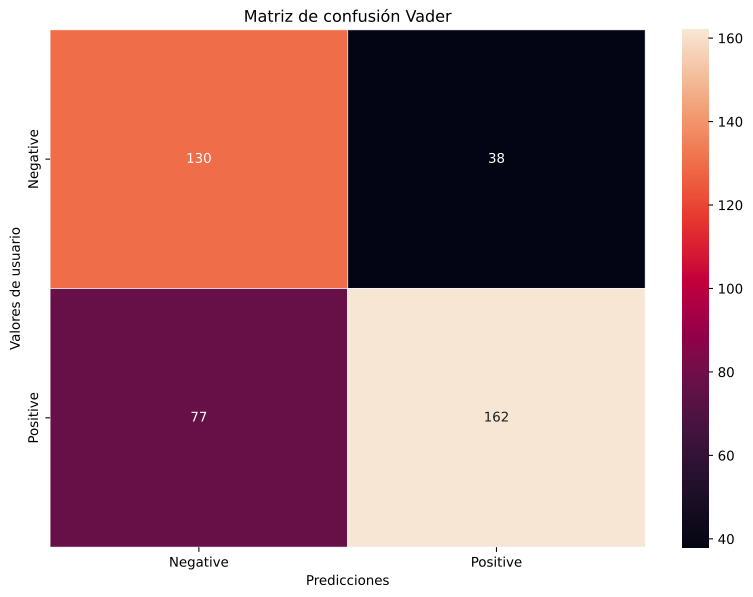
\includegraphics[scale=0.3]{svg/vader_confusion.png}
   \caption{Matriz de confusión Vader sentiment}
\end{figure}

La matriz de confusión representa el número de elementos de cada clase.
Como podemos ver hay 38 casos en los que el modelo ha identificado la 
reseña como positiva cuando en realidad es negativa.
Además hay 77 casos en los que ha identificado un sentimiento positivo 
cuando en realidad es negativo.

\begin{figure}[h]
   \advance\leftskip2cm 
   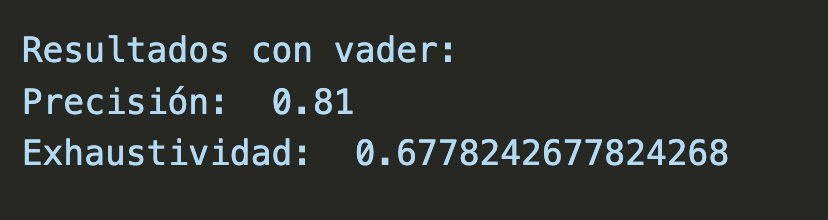
\includegraphics[scale=0.4]{vader_results.png}
   \caption{Resultados Vader Sentiment}
\end{figure}
La precisión representa la proporción de reseñas correctamente identificadas
con respecto al total. Dicho de otra forma el porcentaje de reseñas relevantes.
Por otra parte, la exhaustividad lo que mide es la proporción de reseñas 
identificadas con respecto al total de reseñas que se deberían haber 
clasificado en ese grupo.
Como vemos en los resultados, con Vader Sentiment el 81\% de las reseñas 
identificadas como positivas, eran efectivamente positivas y se ha podido identificar 
el 61\% del total de las reseñas positivas.

\newpage
\subsection{Prompt sentiment}

\begin{figure}[h]
   \advance\leftskip2cm 
   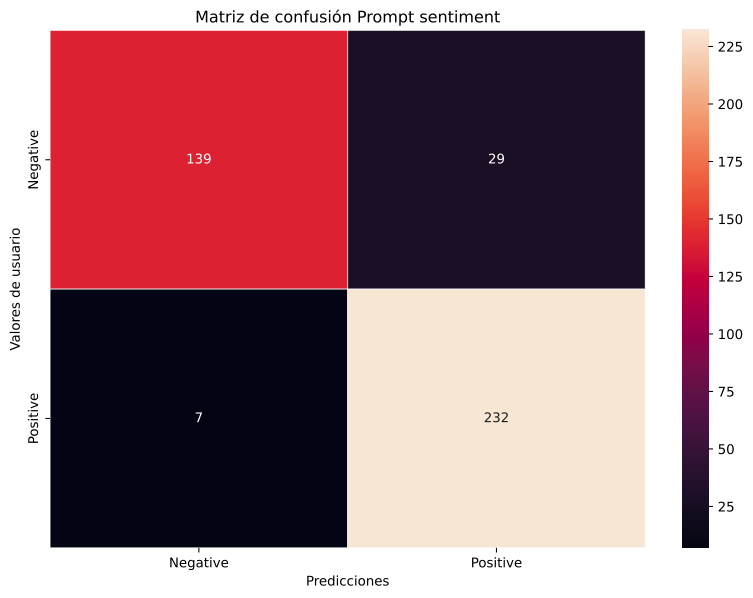
\includegraphics[scale=0.3]{svg/prompt_sentiment_confusion.png}
   \caption{Matriz de confusión Prompt Sentiment}
\end{figure}
Con respecto a nuestro sistema ha identificado 29 reseñas como positivas 
cuando en realidad son negativas y 7 que identificado como negativas 
cuando en realidad son positivas.


\begin{figure}[h]
   \advance\leftskip2cm 
   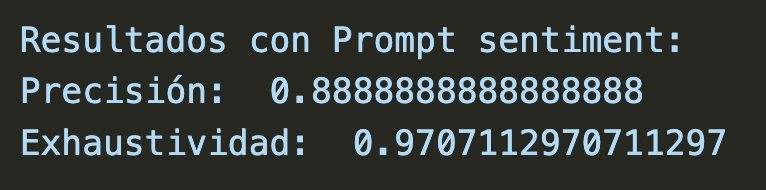
\includegraphics[scale=0.4]{prompt_sentiment_results.png}
   \caption{Resultados Prompt Sentiment}
\end{figure}
En relación a la precisión el 89\% de las reseñas identificadas como positivas eran, efectivamente positivas.
y se ha logrado clasificar correctamente el 97\% de las reseñas positivas.

En vista a estos resultados podemos afirmar que nuestro sistema funciona bastante 
mejor que Vader Sentiment tanto en precisión como en exhaustividad. 
Podemos afirmar que nuestro sistema es indestiguible de un humano clasificando 
reseñas según el sentimiento.



